\chapter{Definitions}
\label{chapter:definitions}

In this chapter we present the definitions and notations used in this work. The definitions shown are based on \cite{BondyNMurty} and \cite{Diestel}.

% Neste capítulo apresentamos as definições e notações usadas nesse trabalho. As definições apresentadas são baseadas em \cite{BondyNMurty} e \cite{Diestel}.

\section{Graphs Notation}

A graph is a pair \(G = (V, E)\) of sets satisfying \(E \subseteq [V]^2\); therefore the elements of \(E\) are subsets of \(V\) with two elements. These two sets can be observed as points and lines connecting points, respectively.

% Um grafo é um par \(G = (V, E)\) de conjunto que satisfazem \(E \subseteq [V]^2\); portanto os elementos de \(E\) são subconjuntos de \(V\) com dois elementos. Esses dois conjuntos podem ser observados como pontos e linhas que conectam pontos, respectivamente.

The set of vertices of a graph is denoted as \(V(G)\) and the set of edges as \(E(G)\). We say that \(v\) belongs to the graph \(G\) following the notation \(v \in V(G)\), and equivalently for an edge \(e\) we denote \(e \in E(G)\). We can also represent vertices and edges using \(v \in G\) or \(e \in G\), in situations where the context clarifies the nature of the treated variable.

% O conjunto de vértices de um grafo é denotado como \(V(G)\) e o conjunto de arestas como \(E(G)\). Dizemos que \(v\) pertence ao grafo \(G\) seguindo a notação \(v \in V(G)\), e de maneira equivalente para uma aresta \(e\) denotamos \(e \in E(G)\). Também podemos representar vértices e arestas usando \(v \in G\) ou \(e \in G\), em situações em que o contexto esclarece a natureza da variável tratada.

A vertex \(v\) is \textbf{incident} to an edge \(e\) if \(v \in e\); so \(e\) is an edge connected to \(v\). The two vertices incident to \(e\) are called the \textbf{endpoints} of \(e\). Another notation used to represent an edge is \(vw \in E(G)\), where \(v, w \in V(G)\) are the endpoints.

% Um vértice \(v\) é \textbf{incidente} a uma aresta \(e\) se \(v \in e\); assim \(e\) é uma aresta conectada à \(v\). Os dois vértices incidentes à \(e\) são chamados de \textbf{extremidades} de \(e\). Outra notação usada para representar uma aresta é \(vw \in E(G)\), onde \(v, w \in V(G)\) são as extremidades. 

The number of vertices of a graph is its \textbf{order}, denoted by \(|G|\). The number of edges is its \textbf{size} and is denoted by \(||G||\).

% O número de vértices de um grafo é a sua \textbf{ordem}, denotado por \(|G|\). O número de arestas é o seu \textbf{tamanho} e é denotado por \(||G||\).

Two vertices \(u\), \(v\) of \(G\) are \textbf{adjacent}, or neighbors, if there is \(e \in E(G)\) such that \(u\) and \(v\) are its endpoints. Two edges \(e\) and \(f\) are adjacent if they have one of their endpoints in common.

% Dois vértices \(u\), \(v\) de \(G\) são \textbf{adjacentes}, ou vizinhos, se existe \(e \in E(G)\) tal que \(u\) e \(v\) são suas extremidades. Duas arestas \(e\) e \(f\) são adjacentes se possuem um dos seus extremos em comum.


Let \(v \in V(G)\) be a vertex. We denote as \(N(v)\) the \textbf{open neighborhood} of \(v\), that is, the set of all vertices \(w \in V(G)\) such that \(w\) is adjacent to \(v\). The \textbf{closed neighborhood} of \(v\), denoted as \(N[v]\) is \(N(v) \cup \{v\}\).

% Seja \(v \in V(G)\) um vértice. Denotamos como \(N(v)\) a \textbf{vizinhança aberta} de \(v\), ou seja, o conjunto de todos vértices \(w \in V(G)\) tal que \(w\) é adjacente à \(v\). A \textbf{vizinhança fechada} de \(v\), denotada como \(N[v]\) é \(N(v) \cup \{v\}\).

If for any vertices \(u, v \in V(G)\) there is an edge \(uv \in E(G)\) then we say that \(G\) is a \textbf{complete} graph. A complete graph of \(n\) vertices is denoted as \(K^n\).

% Se para quaisquer vértices \(u, v \in V(G)\) existe uma aresta \(uv \in E(G)\) então dizemos que \(G\) é um grafo \textbf{completo}. Um grafo de \(n\) vértices completo é denotado como \(K^n\).

The \textbf{degree} of a vertex \(v\) is the number of edges of \(G\) incident to \(v\), denoted by \(d(v)\). Note that \(d(v) = |N(v)|\) if the graph has no loops or multiple edges. Let \(v\) be a vertex such that \(d(v) = 0\), we say that \(v\) is an \textbf{isolated vertex}. The number \(\delta(G) := \min \{d(v) \colon v \in V(G)\}\) is the \textbf{minimum degree} of \(G\), the number \(\Delta(G) := \max \{d(v) \colon v \in V(G)\}\) is the \textbf{maximum degree} of \(G\).

% O \textbf{grau} de um vértice \(v\) é o número de arestas de \(G\) incidentes à \(v\), denotado por \(d(v)\). Note que \(d(v) = |N(v)|\) se o grafo não possui laços nem arestas múltiplas. Seja \(v\) um vértice tal que \(d(v) = 0\), dizemos que \(v\) é um \textbf{vértice isolado}. O número \(\delta(G) := \min \{d(v) \colon v \in V(G)\}\) é o \textbf{grau mínimo} de \(G\), o número \(\Delta(G) := \max \{d(v) \colon v \in V(G)\}\) é o \textbf{grau máximo} de \(G\).

We say that a graph \(H = (V' , E')\) is \textbf{subgraph} of \(G\) if \(V' \subseteq V\) and \(E' \subseteq E\), that is, \(H \subseteq G\). If for any vertices \(v, w \in H \subset G\) the statement \(vw \in E(H)\) is valid if and only if \(vw \in E(G)\), then we say that \(H\) is an \textbf{induced subgraph} of \(G\), and we denote it by \(G[H]\). We say that \(H\) is a \textbf{spanning subgraph} of \(G\) if \(V' = V\).

% Dizemos que um grafo \(H = (V' , E')\) é \textbf{subgrafo} de \(G\) se \(V' \subseteq V\) e \(E' \subseteq E\), ou seja, \(H \subseteq G\). Se para quaisquer vértices \(v, w \in H \subset G\) for válida a afirmação \(vw \in E(H)\) se, e somente se, \(vw \in E(G)\), então dizemos que \(H\) é um \textbf{subgrafo induzido} de \(G\), e o denotamos por \(G[H]\). Dizemos que \(H\) é um \textbf{subgrafo gerador} de \(G\) caso \(V' = V\).

A \textbf{path} in a graph \(G\) is a sequence of distinct vertices \(P = v_1, v_2, \dots, v_k\), \(P \subseteq V(G)\), such that for every pair of consecutive vertices of \(P\), there is an edge in \(E(G)\) that connects these vertices, that is, for every \(v_i , v_{i+1}\) in \(P\), there is \(v_i v _{i+1} \in E(G)\). The number of vertices in the path is its length, and a path of length \(k\) is denoted by \(P^k\).

% Um \textbf{caminho} em um grafo \(G\) é uma sequência de vértices \(P = v_1, v_2, \dots, v_k\) distintos, \(P \subseteq V(G)\), tal que para todo par de vértices consecutivos de \(P\), existe uma aresta em \(E(G)\) que conecta esses vértices, ou seja, para todo \(v_i , v_{i+1}\) em \(P\), existe \(v_i v _{i+1} \in E(G)\). O número de vértices no caminho é o seu comprimento, um caminho de comprimento \(k\) é denominado \(P^k\).

If \(P = v_1, v_2 \dots, v_k\) is a path such that \(|P| \geq 3\) and the endpoints of the sequence \(P\) are equal, that is, \(v_1 = v_k\) , then we say that \(P\) is a \textbf{cycle}. The number of vertices of a cycle is its \textbf{length}, a cycle of length \(k\) is called \(C^k\). However, in this work, we relax the definition of cycle for the sake of simplicity. We define a cycle as a multiset of edges such that every vertex of \(G\), that is endpoint to some edge in the multiset, has even degree considering all edges in the multiset. 

% Se \(P = v_1, v_2 \dots, v_k\)  é um caminho tal que \(|P| \geq 3\) e os extremos da sequência \(P\) são iguais, ou seja, \(v_1 = v_k\) , então dizemos que \(P\) é um \textbf{ciclo}. O número de vértices de um ciclo é o seu \textbf{comprimento}, um ciclo de comprimento \(k\) é denominado \(C^k\). Neste trabalho, a definição de ciclos apresentada será relaxa permitindo a repetição de vértices. Isso é feito a fim de adequar melhor a definição do SMCP.

If there is a partition of \(V(G)\) into subsets \(V_1 , V_2 , \dots, V_w\) such that two vertices \(u\) and \(v\) are connected if, and only if, \(u\) and \(v\) belong to the same subset \(V_i\), then we say that the subgraphs \(G[V_1], G[V_2], \dots, G[V_w]\) are the \textbf{components} of \(G\). If \(G\) contains a single component, we say that \(G\) is \textbf{connected}, otherwise \(G\) is \textbf{disconnected}.

% Se existir uma partição de \(V\) em subconjuntos \(V_1 , V_2 , \dots, V_w\) tal que dois vértices \(u\) e \(v\) estão conectados se, e somente se, \(u\) e \(v\) pertencem ao mesmo subconjunto \(V_i\). Os subgrafos \(G[V_1], G[V_2], \dots, G[V_w]\) são as \textbf{componentes} de \(G\). Se \(G\) contém uma única componente, dizemos que \(G\) é \textbf{conexo}, caso contrário \(G\) é \textbf{desconexo}.

Let \(e \in E(G)\), denote by \(G / e\) the graph obtained from \(G\) by \textbf{contracting} the edge \(e\) at a new vertex \(v_e\), which becomes adjacent to all old neighbors of the endpoint vertices of \(e\).

% Seja \(e \in E(G)\), denotamos por \(G / e\) o grafo obtido a partir de \(G\) ao \textbf{contrair} a aresta \(e\) em um novo vértice \(v_e\), que se torna adjacente a todos os antigos vizinhos dos vértices extremidade de \(e\).

We define \(c \colon E(G) \to \mathbb{R}_\ge\), for \(e \in E(G)\) as the \textbf{cost} of \(e\). Equivalently \(c(H)\) for \(H \subset G\) is the sum of the cost of the edges of the subgraph \(H\). Let \(C = \{v_1, v_2, \dots, v_k\}\) be a cycle of \(G\), and there may be repetition of vertices in \(C\). We define \(c(C) = \sum_{i=1}^{k-1} c(v_i v_{i+1})\). Note that the same edge can be counted more than once in the cost calculation.

% Definimos \(c \colon E(G) \to \mathbb{R}_\ge\), para \(e \in E(G)\) como o \textbf{custo} de \(e\). De maneira equivalente \(c(H)\) para \(H \subset G\) é a soma do custo das arestas do subgrafo \(H\). Seja \(C = \{v_1, v_2, \dots, v_k\}\) um ciclo de \(G\), podendo haver repetição de vértices em \(C\). Definimos \(c(C) = \sum_{i=1}^{k-1} c(v_i v_{i+1})\). Note que uma mesma aresta pode ser contabilizada mais de uma vez no cálculo do custo.

For vertices \(v, w \in V(G)\) we define the distance between vertices $v$ and $w$, denoted by \(dist_G(v, w)\), as the length of the shortest path between \(v\) and \(w\) in \(G\). If such a path does not exist, by convention we consider \(dist_G(v, w) = +\infty\). We generalize the notation for distances between vertices and edges. Let \(v \in V(G)\) and \(uw \in E(G)\) define the distance between the vertex \(v\) and the edge \(uw\) as \(dist_G(v, uw) := \min\{dist_G(v, u), dist_G(v, w)\} + c(uw)\).

% Para vértices \(v, w \in V(G)\) definimos a distância entre os vértices $v$ e $w$, denotado por \(dist_G(v, w)\), como o comprimento do caminho mais curto entre \(v\) e \(w\) em \(G\). Caso tal caminho não exista, por convenção, consideramos \(dist_G(v, w) = +\infty\). Generalizamos a notação para distâncias entre vértices e arestas. Seja \(v \in V(G)\) e \(uw \in E(G)\) definimos a distância entre o vértice \(v\) e a aresta \(uw\) como \(dist_G(v, uw) := \min\{dist_G(v, u), dist_G(v, w)\} + c(uw)\).

We say that a graph \(F\) without cycles is a \textbf{forest}. A connected forest is a \textbf{tree}. Let \(T\) be a tree and \(v \in T\) a vertex, if \(d(v) = 1\), we say that \(v\) is a \textbf{leaf} of \(T \), all other vertices are called inner vertices of \(T\). A tree is rooted if one of its vertices has been chosen as \textbf{root}.

% Dizemos que um grafo \(F\) sem ciclos é uma \textbf{floresta}. Uma floresta conexa é uma \textbf{árvore}. Seja \(T\) uma árvore e \(v \in T\) um vértice, se \(d(v) = 1\), dizemos que \(v\) é uma \textbf{folha} de \(T\), todos demais vértices são chamados de vértices internos de \(T\). Uma árvore é enraizada se um dos seus vértices foi eleito como \textbf{raiz}.

Let \(T\) be a rooted tree with root \(r \in V(T)\), let \(v \in V(T)\), let \(P\) be the path between \(v\) and \(r\). we say that \(w \in V(T)\) is the parent vertex of \(v\) if \(w \in P\) and \(w \in N(v)\). Equivalently, we say that \(v\) is a child vertex of \(w\). Note that a vertex can have multiple children, but only one parent.

% Seja \(T\) uma árvore enraizada com raiz \(r \in V(T)\), seja \(v \in V(T)\), seja \(P\) o caminho entre \(v\) e \(r\). dizemos que \(w \in V(T)\) é o vértice pai de \(v\) se \(w \in P\) e \(w \in N(v)\). De maneira equivalente, dizemos que \(v\) é um vértice filho de \(w\). Note que um vértice pode ter múltiplos filhos, mas somente um pai.

Informally, we say that if a graph \(G\) can be drawn on a plane without its edges intersecting, then it is \textbf{planar}. Thus, the graph can be seen as points on a surface with arcs connecting the points. The surface region completely surrounded by arcs is called \textbf{face} of the graph. In particular, the outer region of the graph is the \textbf{outer face}, while all other faces are \textbf{inner faces} of \(G\). The boundary of \(G\), i.e. the set of edges that separate the outer face of \(G\) from the rest of the graph, is called \(\partial(G)\).

% De maneira informal, dizemos que se um grafo \(G\) é \textbf{planar} se pode ser desenhado em um plano sem que suas arestas se cruzem. Sendo assim, o grafo pode ser visto como pontos em uma superfície com arcos conectando os pontos. A região da superfície completamente circundada de arcos é denominada \textbf{face} do grafo. Em particular, a região exterior do grafo é a \textbf{face externa}, ao passo que todas outras faces são \textbf{faces internas} de \(G\). A fronteira de \(G\), ou seja o conjunto de arestas que separam a face externa de \(G\) do restante do grafo, é denominada \(\partial(G)\).

Formally, \cite{Diestel} defines a planar graph as a pair \((V, E)\) of finite sets with the following properties:

\begin{itemize}
    \item \(V \subseteq \mathbb{R}^2\);
    \item every edge is an arc between two vertices;
    \item different edges have different set of extreme points;
    \item the interior of an edge does not contain vertices or intersections with other edges.
\end{itemize}

% Formalmente, \cite{Diestel} define um grafo planar como um par \((V, E)\) de conjuntos finitos com as seguintes propriedades:

% \begin{itemize}
%     \item \(V \subseteq \mathbb{R}^2\);
%     \item toda aresta é um arco entre dois vértices;
%     \item diferentes arestas tem diferentes conjunto de pontos extremais;
%     \item o interior de uma aresta não contém vértices e nem intersecções com outras arestas.
% \end{itemize}

For any planar graph the set \(\mathbb{R}^2 \backslash G\) is open and its regions are the faces of \(G\).

Informally we say that the \textbf{genus} of a graph is the smallest number \textit{g} such that the graph can be drawn on a sphere with \textit{g} holes without their edges crossing. Therefore, a planar graph has genus 0. The problem of determining the genus of a graph is known to be \(\nonpoly\)-complete, as demonstrated by \cite{THOMASSEN1989568}. However, as presented by \cite{LinearGenus}, the problem becomes treatable with genus \textit{g} fixed, that is, we can determine in polynomial time whether a graph can be embedded in a surface with genus \textit{g}, considering \textit{g} constant.

% Para qualquer grafo planar o conjunto \(\mathbb{R}^2 \backslash G\) é aberto e suas regiões são as faces de \(G\).

% Informalmente dizemos que o \textbf{genus} de um grafo é o menor número \textit{g} tal que o grafo pode ser desenhado em uma esfera com \textit{g} buracos sem que as suas arestas se cruzem. Sendo assim, uma grafo planar tem \textit{genus} 0. Sabe-se que o problema de determinar o \textit{genus} de um grafo é \(\nonpoly\)-completo, como demonstrado por \cite{THOMASSEN1989568}. Entretanto, como apresentado por \cite{LinearGenus}, o problema passa a ser tratável com \textit{genus} \textit{g} fixo, ou seja, podemos determinar em tempo polinomial se um grafo pode ser incorporada em uma superfície com \textit{genus} \textit{g}, considerando \textit{g} constante.

For a given planar graph \(G\) we say that \(H\) is its \textbf{dual} if there is a bijective function that maps the faces of \(G\) to the vertices of \(H\). Furthermore, for each edge \(e \in E(G)\) that separates the faces \(f\) and \(f'\) of \(G\), we have an edge that connects the vertices referring to \(f\) and \(f'\) in \(H\).

% Para um dado grafo planar \(G\) dizemos que \(H\) é seu \textbf{dual} se existe uma função bijectiva que mapeia as faces de \(G\) à vértices de \(H\). Além disso, para cada aresta \(e \in E(G)\) que separa as faces \(f\) e \(f'\) de \(G\), temos uma aresta que conecta os vértices referentes à \(f\) e \(f'\) em \(H\) .

As defined by \cite{ROBERTSON1986309}, a \textbf{tree decomposition} of \(G\) is a pair \((T, B)\) in which \(T\) is a tree and \(B = \{B_i \colon i \in V(T)\}\) is a family of subsets of \(V(G)\) such that:

\begin{itemize}
    \item \(\bigcup_{i \in V(T)} B_i = V(G)\)
    \item For each edge \(uv \in E(G)\), there is \(i \in V(T)\) such that \(u, v \in B_i\)
    \item The set of vertices \(\{i \in V(T) \colon v \in B_i\}\) forms a subtree of \(T\) for each \(v \in V(G)\)
\end{itemize}

% Conforme definida por \cite{ROBERTSON1986309}, uma \textbf{decomposição em árvore} de \(G\) é um par \((T, B)\) no qual \(T\) é uma árvore e \(B = \{B_i \colon i \in V(T)\}\) é uma família de subconjuntos de \(V(G)\) tal que:

% \begin{itemize}
%     \item \(\bigcup_{i \in V(T)} B_i = V(G)\)
%     \item Para cada aresta \(uv \in E(G)\), existe \(i \in V(T)\) tal que \(u, v \in B_i\)
%     \item O conjunto de vértices \(\{i \in V(T) \colon v \in B_i\}\) formam uma subárvore de \(T\) para cada \(v \in V(G)\)
% \end{itemize}

To differentiate from the original graph \(G\), we call the vertices of \(T\) \textbf{nodes}, where each node \(i\) has a \textbf{bag} of vertices \(B_i\) corresponding. An example can be seen in Figure \ref{fig:decomp1} where Item (a) is a graph and (b) is a possible tree decomposition for the graph.

% Para diferenciar do grafo original \(G\), chamamos os vértices de \(T\) de \textbf{nós}, onde cada nó \(i\) possui uma \textbf{sacola} de vértices, ou simplesmente \textit{bag}, \(B_i\) correspondente. Um exemplo pode ser observado na Figura \ref{fig:decomp1} onde o Item (a) é um grafo e (b) é uma possível decomposição em árvore para o grafo.

\begin{figure}[H]
    \centering
    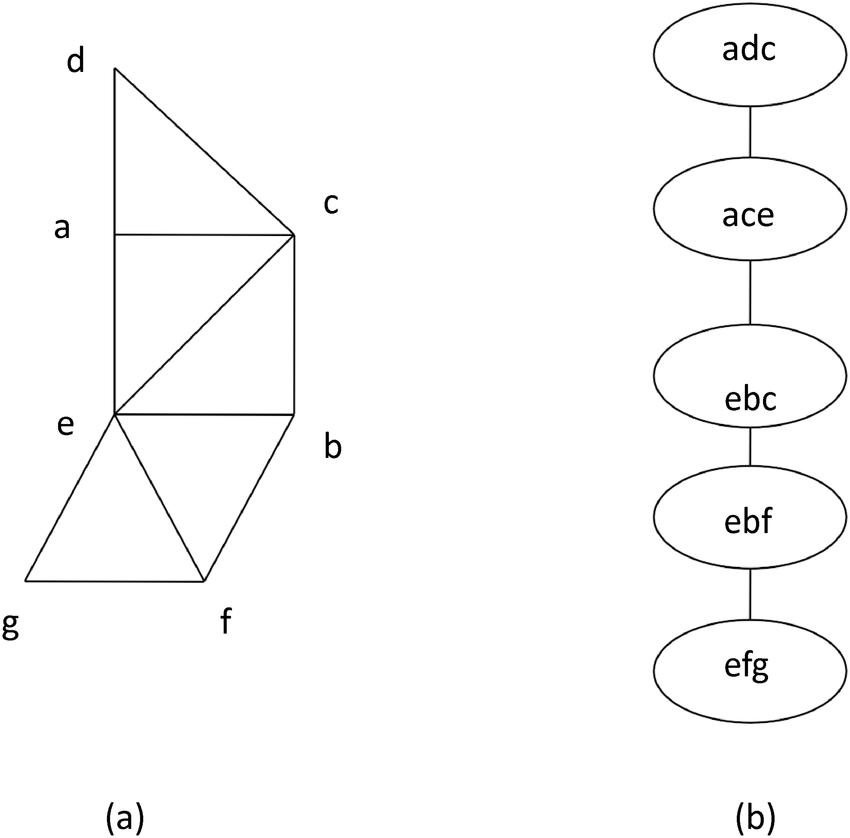
\includegraphics[scale=2]{imgs/decomp1.png}
    \caption{Example of graph and its tree decomposition. (\cite{imgTreeDecomp}).}
    \label{fig:decomp1}
\end{figure}

\begin{tikzpicture}

\Vertex[x=0, y=0, label=$g$, position=below, color=white, size=0.5]{G}
\Vertex[x=1, y=0, label=$f$, position=below, color=white, size=0.5]{F}
\Vertex[x=0.5, y=1, label=$e$, position=left, color=white, size=0.5]{E}
\Vertex[x=1.5, y=1, label=$b$, position=right, color=white, size=0.5]{B}
\Vertex[x=0.5, y=2, label=$a$, position=left, color=white, size=0.5]{A}
\Vertex[x=1.5, y=2, label=$c$, position=right, color=white, size=0.5]{C}
\Vertex[x=0.5, y=3, label=$d$, position=left, color=white, size=0.5]{D}

\Edge(A)(C)
\Edge(A)(D)
\Edge(A)(E)
\Edge(B)(C)
\Edge(B)(E)
\Edge(B)(F)
\Edge(C)(D)
\Edge(E)(F)
\Edge(E)(G)
\Edge(F)(G)

\end{tikzpicture}

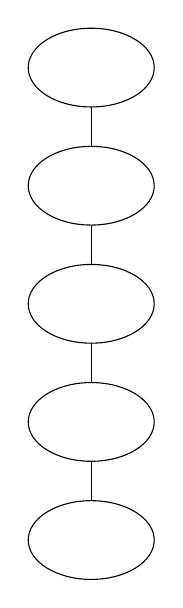
\begin{tikzpicture}

\draw[label=$a$] (0, 0) ellipse (.8 and 0.5);
\draw (0, 1.5) ellipse (.8 and 0.5);
\draw (0, 3) ellipse (.8 and 0.5);
\draw (0, 4.5) ellipse (.8 and 0.5);
\draw (0, 6) ellipse (.8 and 0.5);

\draw (0, 0.5) -- (0, 1);
\draw (0, 2) -- (0, 2.5);
\draw (0, 3.5) -- (0, 4);
\draw (0, 5) -- (0, 5.5);

\end{tikzpicture}

% usar subfigures para colocar as imagens um do lado do outro

The \textbf{width} of a tree decomposition is the size of its largest bag minus one. The \textbf{tree width} of a graph \(G\), denoted with \(tw(G)\), is the smallest width of a tree decomposition of \(G\).

To facilitate application in algorithms, we focus on a more restricted class of decompositions. We say that a tree decomposition \((T, B)\) is \textbf{nice} when \(T\) is a rooted tree and each \(i \in V(T)\) belongs to one of the following classes:

% A \textbf{largura} de uma decomposição em árvore é o tamanho da sua maior sacola menos um. A \textbf{largura de árvore}, ou largura arbórea, de um grafo \(G\),  denotada com \(tw(G)\), é a menor largura de uma decomposição arvórea de \(G\).

% Para facilitar a aplicação em algoritmos, focamos em uma classe mais restrita de decomposições. Dizemos que uma decomposição em árvore \((T, B)\) é agradável, ou \textit{nice}, quando \(T\) é uma árvore enraizada e cada \(i \in V(T)\) pertence a uma das seguintes classes:

\begin{itemize}
    \item \(i\) is a leaf node if it has no children;
    \item \(i\) is a union node if \(i\) has exactly two children \(i_1, i_2\) and is worth \(B_i = B_1 = B_2\);
    \item \(i\) is an introduction node if it has a single child \(i'\) and is valid \(B_i = B_{i'} \cup \{v\}\) for some vertex \(v \in V(G)\);
    \item \(i\) is a forgetting node if it has a single child \(i'\) and holds \(B_i = B_{i'} \backslash \{v\}\) for some vertex \(v \in V(G)\).
\end{itemize}

% \begin{itemize}
%     \item \(i\) é um nó folha se não tiver nenhum filho;
%     \item \(i\) é um nó de união se \(i\) tiver exatamente dois filhos \(i_1, i_2\) e vale \(B_i = B_1 = B_2\);
%     \item \(i\) é um nó de introdução se tiver um único filho \(i'\) e vale \(B_i = B_{i'} \cup \{v\}\) para algum vértice \(v \in V(G)\);
%     \item \(i\) é um nó de esquecimento se tiver um único filho \(i'\) e vale \(B_i = B_{i'} \backslash \{v\}\) para algum vértice \(v \in V(G)\);
% \end{itemize}

\section{Classes of Optimization Problems}

In combinatorial optimization problems, we want to obtain the best solution out of a finite, but potentially large, set of possible solutions. \cite{livroAprox} defined an optimization problem with the following elements: a set of instances, a set \(\sol(I)\) of viable solutions for a given instance \(I\) and a function \(\val (I, S)\) that associates for each instance and solution \(S \in \sol(I)\) a non-negative rational value. Therefore, the solution to the optimization problem is the \(S\) that minimizes/maximizes \(\val(I, S)\).

% Em problemas de otimização combinatória, desejamos obter a melhor solução dentro de um conjunto finito, mas potencialmente grande, de soluções possíveis. \cite{livroAprox} definiram um problema de otimização com os seguintes elementos: um conjunto de instâncias, um conjunto \(\sol(I)\) de soluções viáveis para uma dada instância \(I\) e uma função \(\val(I, S)\) que associa para cada instância e solução \(S \in \sol(I)\) um valor racional não-negativo. Sendo assim, a solução do problema de otimização é o \(S\) que minimiza/maximiza \(\val(I, S)\).


More formally, for a given instance \(I\) there is a solution \(S^* \in \sol(I)\) such that \(\val(I, S^*) \leq \val(I, S)\) for all \(S \in \sol(I)\), considering a minimization scenario. The idea follows in an equivalent way for a maximization problem. We denote \(\opt := \val(I, S^*)\) as the optimal solution of \(I\). In particular, for the problems discussed in this work, we denote as \(\opt_{\mathcal{T}}(G)\) an optimal solution in the graph \(G\) considering a set of pairs of terminals \(\mathcal{T}\).

% Mais formalmente, para uma dada instância \(I\) existe uma solução \(S^* \in \sol(I)\) tal que \(\val(I, S^*) \leq \val(I, S)\) para todo \(S \in \sol(I)\), considerando um cenário de minimização. A ideia segue de maneira equivalente para um problema de maximização. Denotamos \(\opt := \val(I, S^*)\) como a solução ótima de \(I\). Em particular, para os problemas comentados nesse trabalho, denotamos como \(\opt_{\mathcal{T}}(G)\) uma solução ótima no grafo \(G\) considerando um conjunto de pares de terminais \(\mathcal{T}\).

As will be seen throughout the section, there is an intimate relationship between the classes of optimization problems and the well-known classes of decision problems: \(\poly\), \(\nonpoly\), \(\nonpoly\)-hard, \(\nonpoly\)-complete. There are optimization problems in which there is limitations of the approximability of their solutions by polynomial algorithms, considering \(\poly \neq \nonpoly\).

% Como será observado ao longo da seção, existe uma relação íntima entre as classes de problemas de otimização e as conhecidas classes de problemas de decisão: \(\poly\), \(\nonpoly\), \(\nonpoly\)-difícil, \(\nonpoly\)-completo. Existem problemas de otimização em que aparecem limitações da aproximalidade de suas soluções por algoritmos polinomiais, considerando \(\poly \neq \nonpoly\).

In this way, optimization problems are classified according to their degree of approximability. When talking about approximation, we are observing a scenario in which we give up finding the optimal solution in favor of finding a solution efficiently, while maintaining quality guarantees. In this work we will consider and detail the classes PO, FPTAS, PTAS, APX and NPO, as described by \cite{bookAprox}.

% Dessa forma, problemas de otimização são classificados conforme seu grau de aproximabilidade. Ao falar de aproximabilidade, estamos observando um cenário em que abrimos mão de encontrar a solução ótima para uma dada instância em favor de encontrar uma solução de maneira eficiente, mas mantendo garantias de qualidade. Neste trabalho vamos considerar e detalhar as classes PO, FPTAS, PTAS, APX e NPO, conforme descrito por \cite{livroAprox}.

According to \citeauthor{bookAprox}, the NPO class, which is an extension of the \(\nonpoly\) class for optimization problems, is composed of the problems where:

\begin{itemize}
    \item There is a polynomial function \textit{p} such that \(\langle S \rangle \leq p\langle\langle I\rangle\rangle\) for every instance \(I\) of the problem and every feasible solution \( S\) of \(I\);
    \item There is a polynomial algorithm that decides whether a given word is a valid representation of an instance of the problem;
    \item There is a polynomial algorithm that decides whether a given object is a viable solution for a given instance of the problem;
    \item There is a polynomial algorithm that calculates \(\val(I, S)\), given \(I\) and \(S\).
\end{itemize}

% De acordo com \citeauthor{livroAprox}, a classe NPO, que é uma extenção da classe \(\nonpoly\) para problemas de otimização, é composta pelos problemas em que:

% \begin{itemize}
%     \item Existe uma função polinomial \textit{p} tal que \(\langle S \rangle \leq p\langle\langle I\rangle\rangle\) para toda instância \(I\) do problema e toda solução viável \(S\) de \(I\);
%     \item Existe uma algoritmo polinomial que decide se uma dada palavra é uma representação válida de uma instância do problema;
%     \item Existe um algoritmo polinomial que decide se um dado objeto é solução viável de uma dada instância do problema;
%     \item Existe um algoritmo polinomial que calcula \(\val(I, S)\), dados \(I\) e \(S\).
% \end{itemize}

We denote as PO the class of problems treatable in polynomial time. This class is an extension of the P class for optimization problems. Therefore, given a problem \(\pi\), we say that \(\pi \in PO\) if there is a polynomial algorithm that calculates an optimal solution for each instance \(I\) of \(\pi\). Examples of problems of this class are the Shortest Path and Minimum Spanning Tree problems.

% Denotamos como PO a classe de problemas tratáveis em tempo polinomial. Esta classe é uma extensão da classe P para problemas de otimização. Sendo assim, dado um problema \(\pi\), dizemos que \(\pi \in PO\) se existe um algoritmo polinomial que calcular uma solução ótima para cada instância \(I\) de \(\pi\). Exemplos de problemas dessa classe são os problemas de Caminho Mínimo e de Árvore Geradora Mínima.

Consider an optimization problem. Let \(A\) be an algorithm in which for every viable instance \(I\) of the problem returns a viable solution \(A(I)\) of \(I\). If the problem is one of minimization and \(A(I) \leq \alpha \opt\) holds for every instance \(I\), then we say that \(A\) is a \(\alpha\)-approximation of the problem. We denote \(\alpha\) as \textbf{approximation ratio} of the algorithm.

% Considere um problema de otimização. Seja \(A\) um algoritmo em que para toda instância \(I\) viável do problema devolve uma solução viável \(A(I)\) de \(I\). Se o problema é de minimização e vale \(A(I) \leq \alpha \opt\) para toda instância \(I\), então dizemos que \(A\) é uma \(\alpha\)-aproximação do problema. Denotamos \(\alpha\) como \textbf{razão de aproximação} do algoritmo.

The APX class is composed of optimization problems in NPO for which there is a \(\alpha\)-polynomial-time approximation for some constant \(\alpha\). One of the most famous algorithms that provides this type of approximation is the Christofides Algorithm, developed by \cite{Christofides2022WorstCaseAO} to the TSP problem restricted to metric graphs and which guarantees an approximation with \(\alpha = 1.5\).

% A classe APX é composta por problemas de otimização em NPO para os quais existe uma \(\alpha\)-aproximação em tempo polinomial para alguma constante \(\alpha\). Um dos algoritmos mais famosos que fornece esse tipo de aproximação é o Algoritmo de Christofides, desenvolvido por \cite{Christofides2022WorstCaseAO} e que garante uma aproximação com \(\alpha = 1,5\) para o problema do TSP restrito à grafos métricos.

For a given optimization problem, we define as an \textbf{approximation scheme} an algorithm that receives an instance \(I\) of the problem as well as a parameter \(0 < \ epsilon < 1\) and returns a solution \(S\) such that \(\val(I, S) \leq (1 + \epsilon) \opt\), for a minimization problem. We say that an algorithm is a \textbf{polynomial-time approximation scheme} (PTAS), if it is polynomial for every fixed \(\epsilon\). Furthermore, an algorithm is a \textbf{full polynomial-time approximation scheme}, or FPTAS, if it is also polynomial in \(1 / \epsilon\), whereas a PTAS algorithm, which is not FPTAS, is exponential in \(1 / \epsilon\).

% Para um dado problema de otimização, definimos como um \textbf{esquema de aproximação}, ou do inglês \textit{approximation scheme}, um algoritmo que recebe uma instância \(I\) do problema assim como um parâmetro \(0 < \epsilon < 1\) e retorna uma solução \(S\) tal que \(\val(I, S) \leq (1 + \epsilon) \opt\), para um problema de minimização. Dizemos que um algoritmo é um \textbf{esquema de aproximação em tempo polinomial}, ou \textit{polynomial-time approximation scheme} (PTAS), se ele é polinomial para todo \(\epsilon\) fixo. Além disso, um algoritmo é um \textbf{esquema de aproximação em tempo polinomial pleno}, ou FPTAS, se ele também é polinomial em \(1 / \epsilon\), ao passo que um algoritmo PTAS, mas não FPTAS, é exponencial em \(1 / \epsilon\).

From the definitions it follows that $$PO \subseteq FPTAS \subseteq PTAS \subseteq APX \subseteq NPO.$$

Equivalent to decision problems, we also have the idea of a problem being NPO-hard, that is, \(PO = NPO\) if and only if \(\poly = \nonpoly\). Therefore, a problem is NPO-hard if it is NPO and its decision version is \(\nonpoly\)-complete. So we have the concept of the \textbf{inapproximability} of a problem.

% De maneira equivalente a problemas de decisão, também temos a ideia de um problema ser NPO-difícil, ou seja \(PO = NPO\) se e somente se \(\poly = \nonpoly\). Sendo assim, um problema é NPO-difícil se for NPO e sua versão de decisão for \(\nonpoly\)-completo. Assim temos o conceito da \textbf{inaproximabilidade} de um problema.

Despite belonging to APX when restricted to metric graphs, the TSP problem is NPO-hard in general graphs. That is, if TSP is in APX, then \(\poly = \nonpoly\). This result has been observed and demonstrated for TSP, and other problems of interest, in \cite{NPOcompleteApproxProblems}.

Equivalently, we also observe APX-hard problems, i.e. if \(\poly = \nonpoly\) then PO = NPO, as noted by \cite{ComplexityApproximation}.

% Apesar de pertencer à APX quando restrito a grafos métricos, o problema TSP é NPO-difícil em grafos gerais. Ou seja se TSP está em APX, então \(\poly = \nonpoly\). Esse resultado foi observado e demonstrado para o TSP, e outros problemas de interesse, em \cite{NPOcompleteApproxProblems}.

% De maneira equivalente, também observamos problemas APX-difíceis. Vale notar que se \(\poly = \nonpoly\) então PO = NPO, conforme observado por \cite{ComplexityApproximation}.
